% !TEX encoding = UTF-8
% !TEX TS-program = pdflatex
% !TEX root = ../tesi.tex
\null\newpage
%**************************************************************
\chapter{Progettazione}
\label{cap:progettazione}
%**************************************************************

\intro{Questo capitolo illustra le caratteristiche dell'applicazione già esistente e lo studio eseguito per comprenderle e motivare le progettuali adottate nello sviluppo del prototipo da me realizzato durante l'esperienza di stage.}\\ %TODO oppure illustra lo stato dell'applicazione

\section{Architettura preesistente}
Trattandosi di effettuare la re-implementazione di una funzionalità preesistente, il primo ostacolo è stato quello di capire come il mio prodotto dovesse integrarsi con il resto dell'architettura cui avrebbe fatto parte, per questo motivo la prima settimana di stage è stata dedicata quasi esclusivamente alla conoscenza dell'ambiente e delle componenti. \\

\subsection{Visione generale}


la figura \ref{schema-generale} illustra, ad alto livello, le relazioni che intercorrono tra le varie tecnologie utilizzate dal software JGalileo CRM.\\
Partendo dalle basi di dati fino ad arrivare all'interfaccia utente, l'architettura del sistema si snoda nel seguente modo:\\
Entrambe le basi di dati, sia quella contenuta nel database del sistema operativo AS400 che quella contenuta sul server, si interfacciano con il \gls{middleware} Hibernate per creare delle classi, equivalenti alle tabelle del database, con cui permettere l'interazione.\\ 
La sezione dell'appendice ~\ref{sec:appendice-1} riporta più nel dettaglio come vengono create le entità Hibernate.\\

\newpage

\begin{figure}[h]
	\centering
	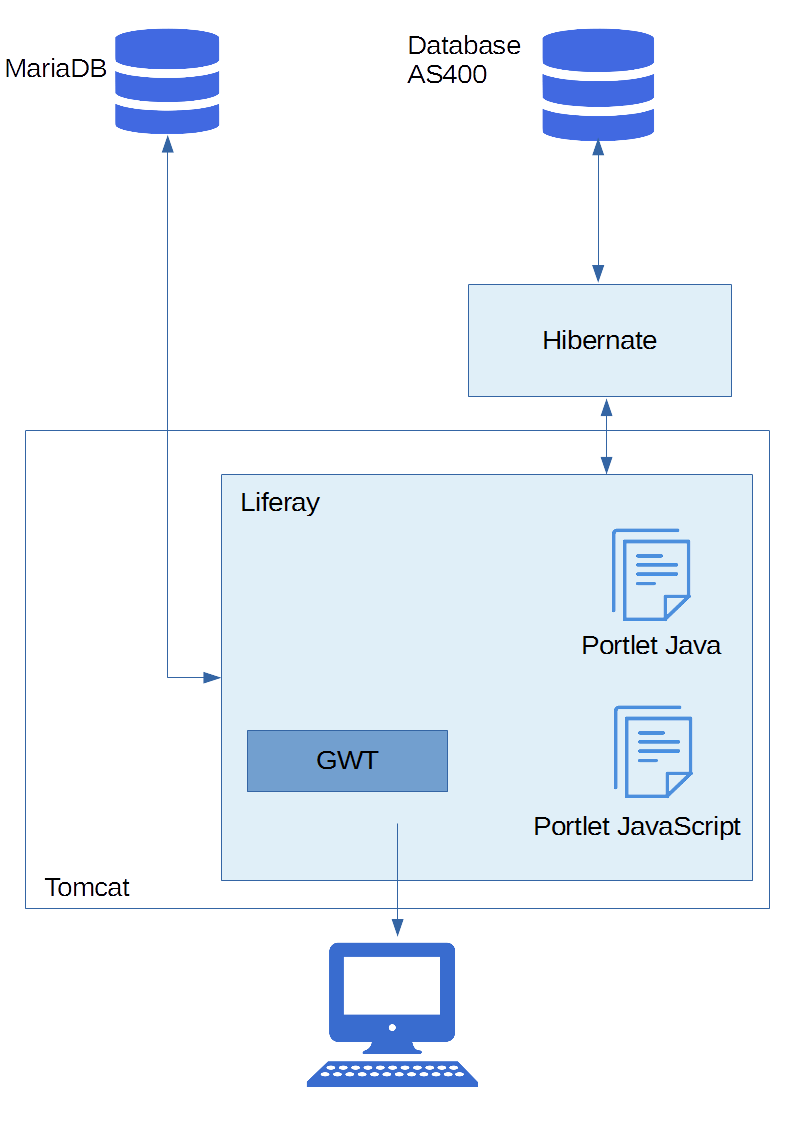
\includegraphics[height = 10 cm]{schema-generale}
	\caption{Schema generale di interconnessione tra le componenti}
	\label{schema-generale}
\end{figure}
L'interazione con le entità di Hibernate avviene per mezzo di Liferay, che si occupa anche della gestione degli accessi degli utenti alla pagina, introducendo il concetto di Single Sing On, e della corretta visualizzazione delle \gls{portlet} all'interno delle pagine del portale. Queste sono caricate di volta in volta, tramite dei servizi \gls{rest}\glsfirstoccur, dal server Tomcat e possono essere scritte in AngularJS, come ad esempio la \gls{portlet} per la geolocalizzazione o quella che gestisce la timeline, oppure in Java per essere successivamente tradotte in JavaScript tramite i servizi offerti da GWT.\\
Le azioni dell'utente vengono gestite poi da Liferay, che si occupa anche del routing tra le varie pagine del portale. Nel caso ci fossero dei dati da salvare, come nel caso dell'inserimento di un nuovo lead, vengono lanciati dei servizi \gls{restg}che andranno ad interfacciarsi con le entità gestite da Hibernate, il quale gestisce la persistenza dei dati.\\

\subsection{Portlet life cycle}
Al fine di capire al meglio come progettare la nuova form, mi sono concentrato sullo studio del ciclo di vita di una \gls{portlet}\hyperlink{24}{[24]}:\\
L'ambiente in cui una essa viene creata ed utilizzata è denominato \emph{portlet container} che, come suggerisce la parola, è un contenitore che gestisce l'aggregazione tra le \gls{portlet}, mantiene memoria delle preferenze dettate dall'utente su di esse ed inoltre funge da \emph{Controller} tra l'interfaccia utente(\emph{View}) ed i dati (\emph{Model}) nel paradigma di programmazione MVC (Model View Controller), illustrato nella sezione ~\ref{sec:MVC}.\\
\newpage
\begin{figure}[h]
	\centering
	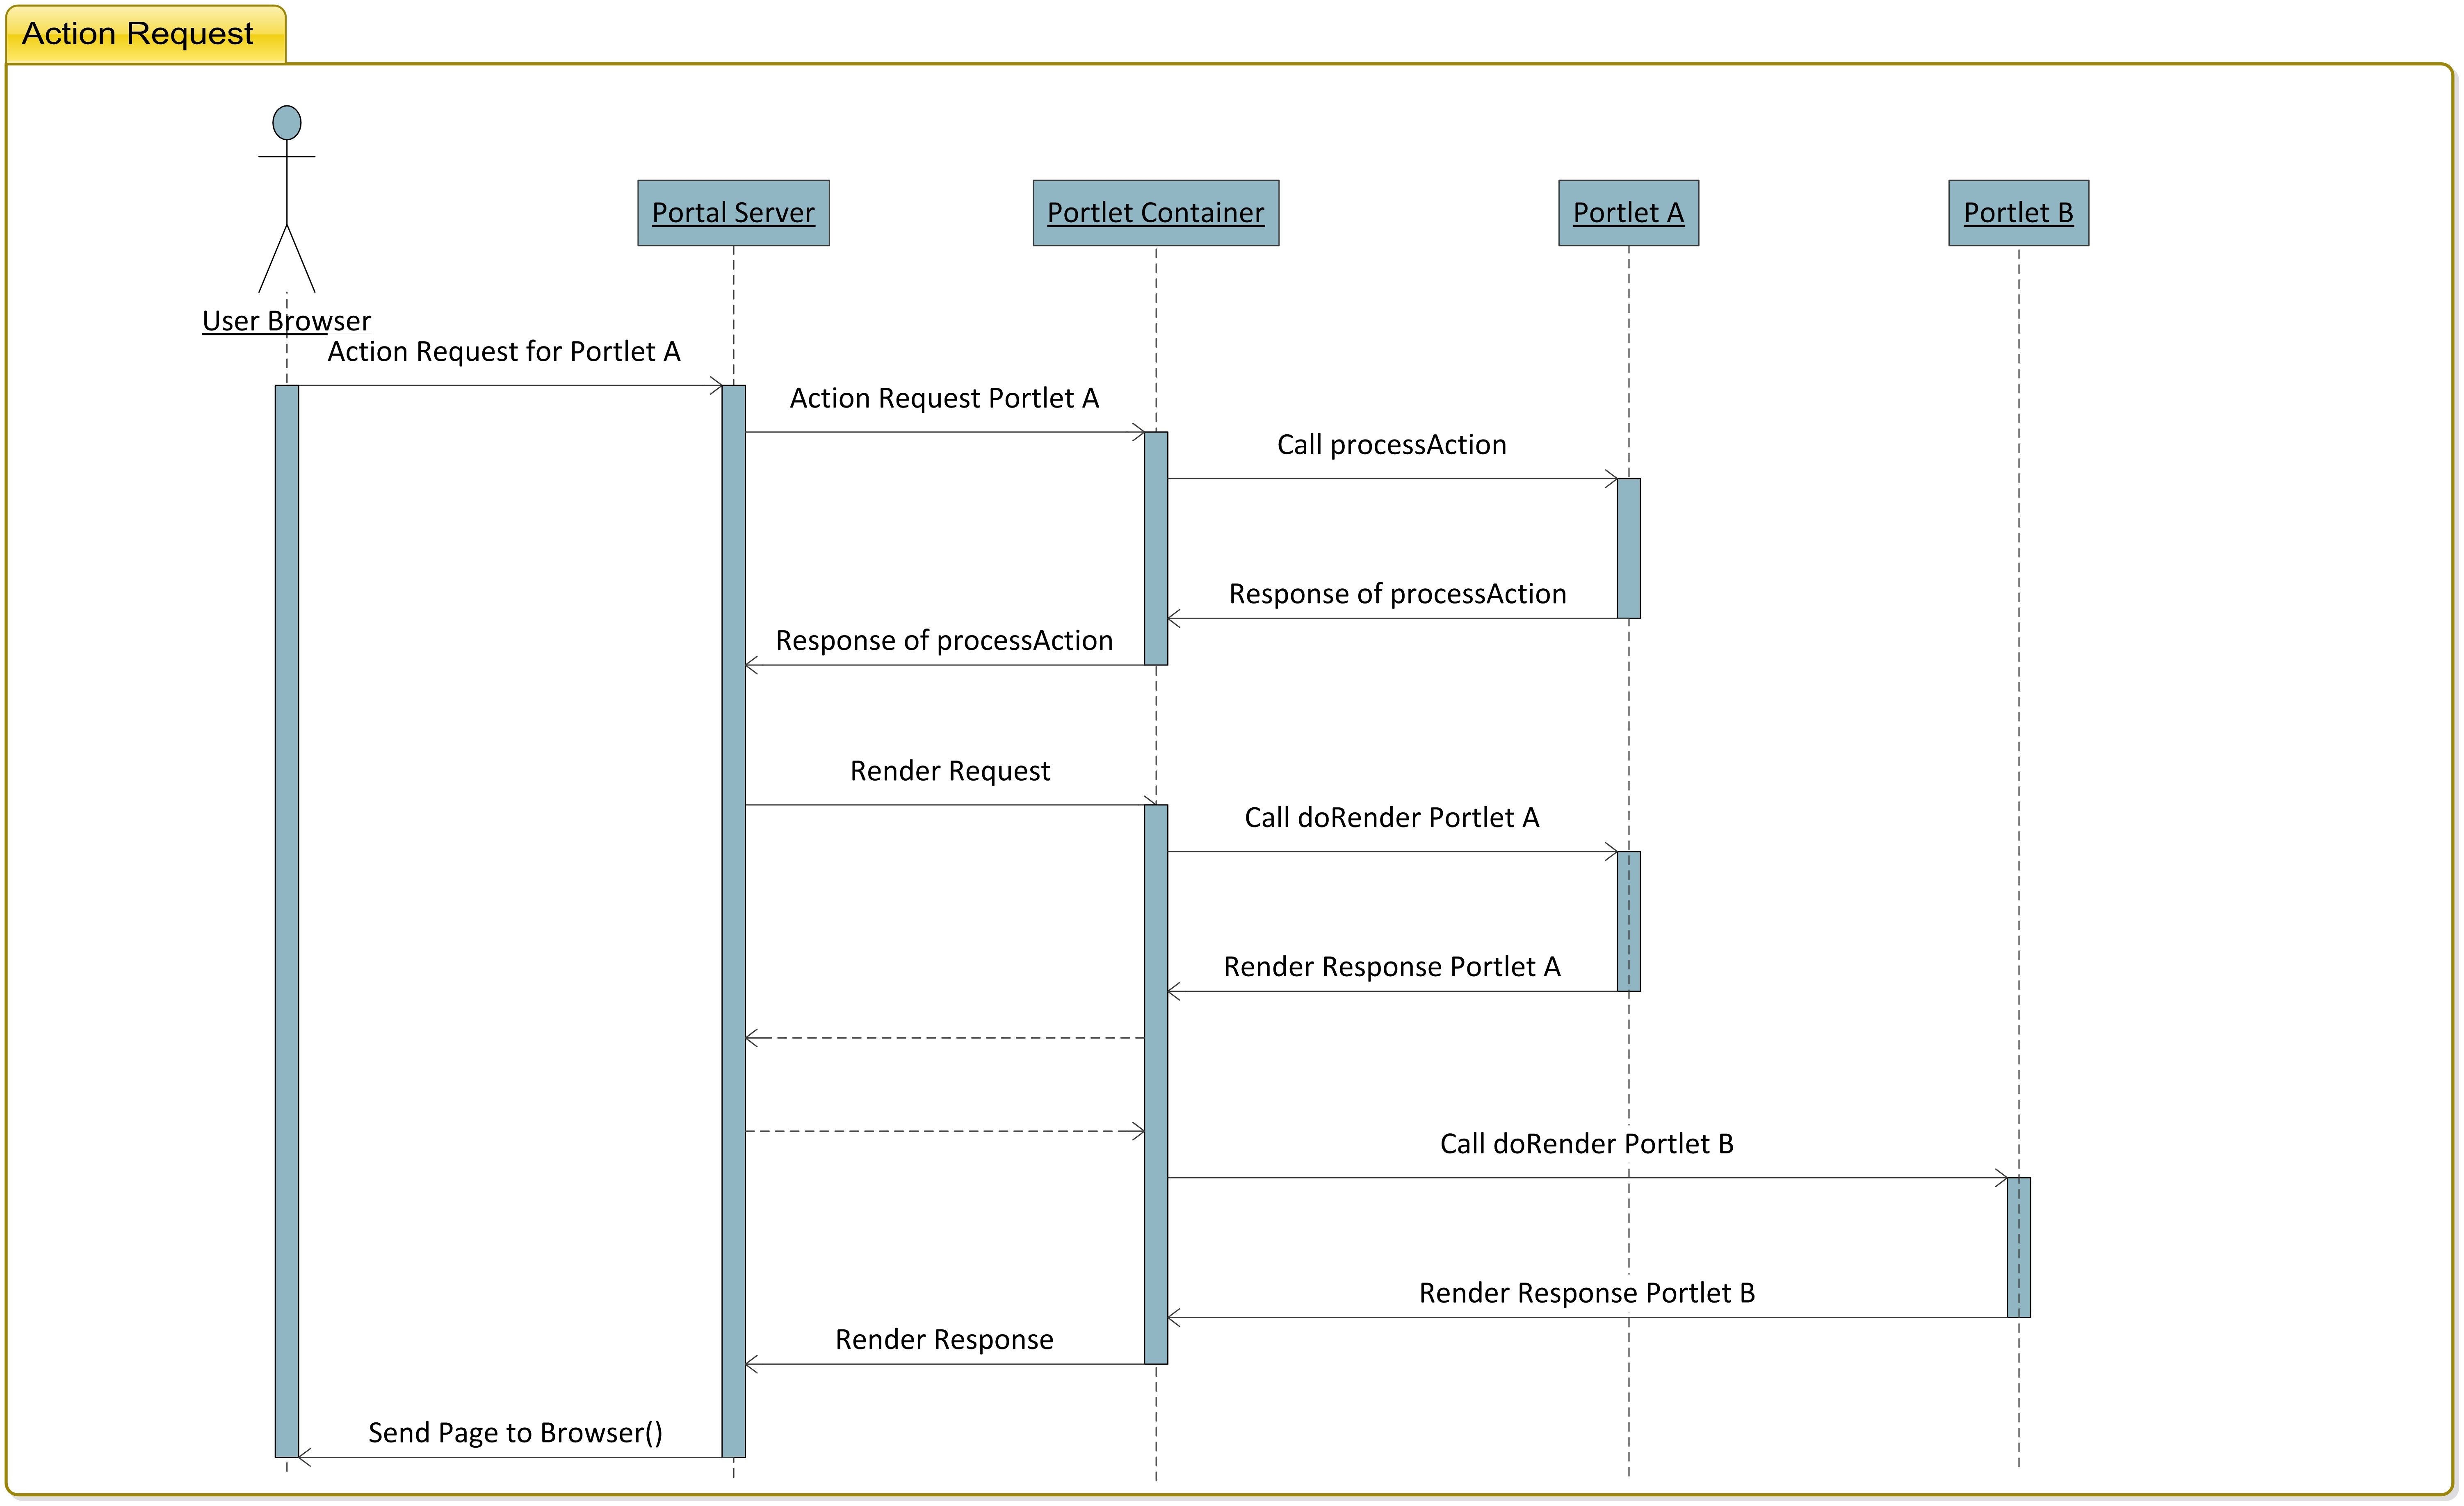
\includegraphics[height = 8 cm]{portet_action_request}
	\caption{Diagramma di sequenza di ProcessAction}
	\label{process-action}
\end{figure}

Il ciclo di vita di una \gls{portlet} è caratterizzato da 6 metodi principali che lo regolano:
\begin{itemize}
	\item \textbf{init()}: chiamato dal portlet container, questo metodo crea la \gls{portlet} desiderata. Durante il ciclo di vita della stassa viene invocato una sola volta;
	\item \textbf{render()}: questo metodo è responsabile della generazione di codice \gls{html} che sarà quindi visualizzato a schermo. Ci sono alcune restrizioni di sicurezza, viene impedita ad esempio la generazione di tag quali <html>, <head>, <body>, che andrebbero a rompere l'intera pagina.
	\item \textbf{processAction()}: processAction viene invocato quando viene eseguita un'azione, ad esempio l'azione di salvataggio di una form. dopo processAction viene automaticamente invocato il metodo render() della \gls{portlet} e delle altre \gls{portlet}, qualora ve ne fossero.
	\item \textbf{processEvent()}: utilizzato per gestire gli eventi, viene poi chiamato il metodo render() della sola \gls{portlet} interessata;
	\item \textbf{serveRescource()}: metodo utilizzato per reperire risorse utilizzando un \gls{urlg};
	\item \textbf{destroy()}: distrugge la \gls{portlet};
\end{itemize}	
\newpage
\section{Form portlet}
La form la cui reimplementazione costituisce il mio progetto di stage consiste in un unica \gls{portlet}, scritta in Java. \\
La \gls{portlet} è costituita da una grande classe, di oltre 6.000 linee di codice, che si appoggia poi ad altre classi per la gestione di aspetti più particolari: ad esempio i campi di tipo picker, cioè dei campi di ricerca che recuperano le voci su cui effettuarla dal database, è separata e lunga circa 4.000 linee di codice.\\
Data l'estrema lunghezza, in rapporto alla mia esperienza di studente, ed alla mancanza di documentazione dovuta all'adozione della metodologia agile, lo studio del funzionamento della \gls{portlet} che gestisce la form ha richiesto più tempo del previsto. \\ 
L'analisi ha portato allo sviluppo del diagramma di flusso riguardante la creazione della \gls{portlet}, illustrato nelle figure \ref{form-portlet-flow-diagram-1} e \ref{form-portlet-flow-diagram-2}. Il diagramma è molto generale a causa della grande complessità di metodi e alternative dettate dal fatto che la form viene creata dinamicamente e deve quindi coprire tutte le possibili casistiche in cui è possibile incorrere.\\

\begin{figure}[p]
	\centering
	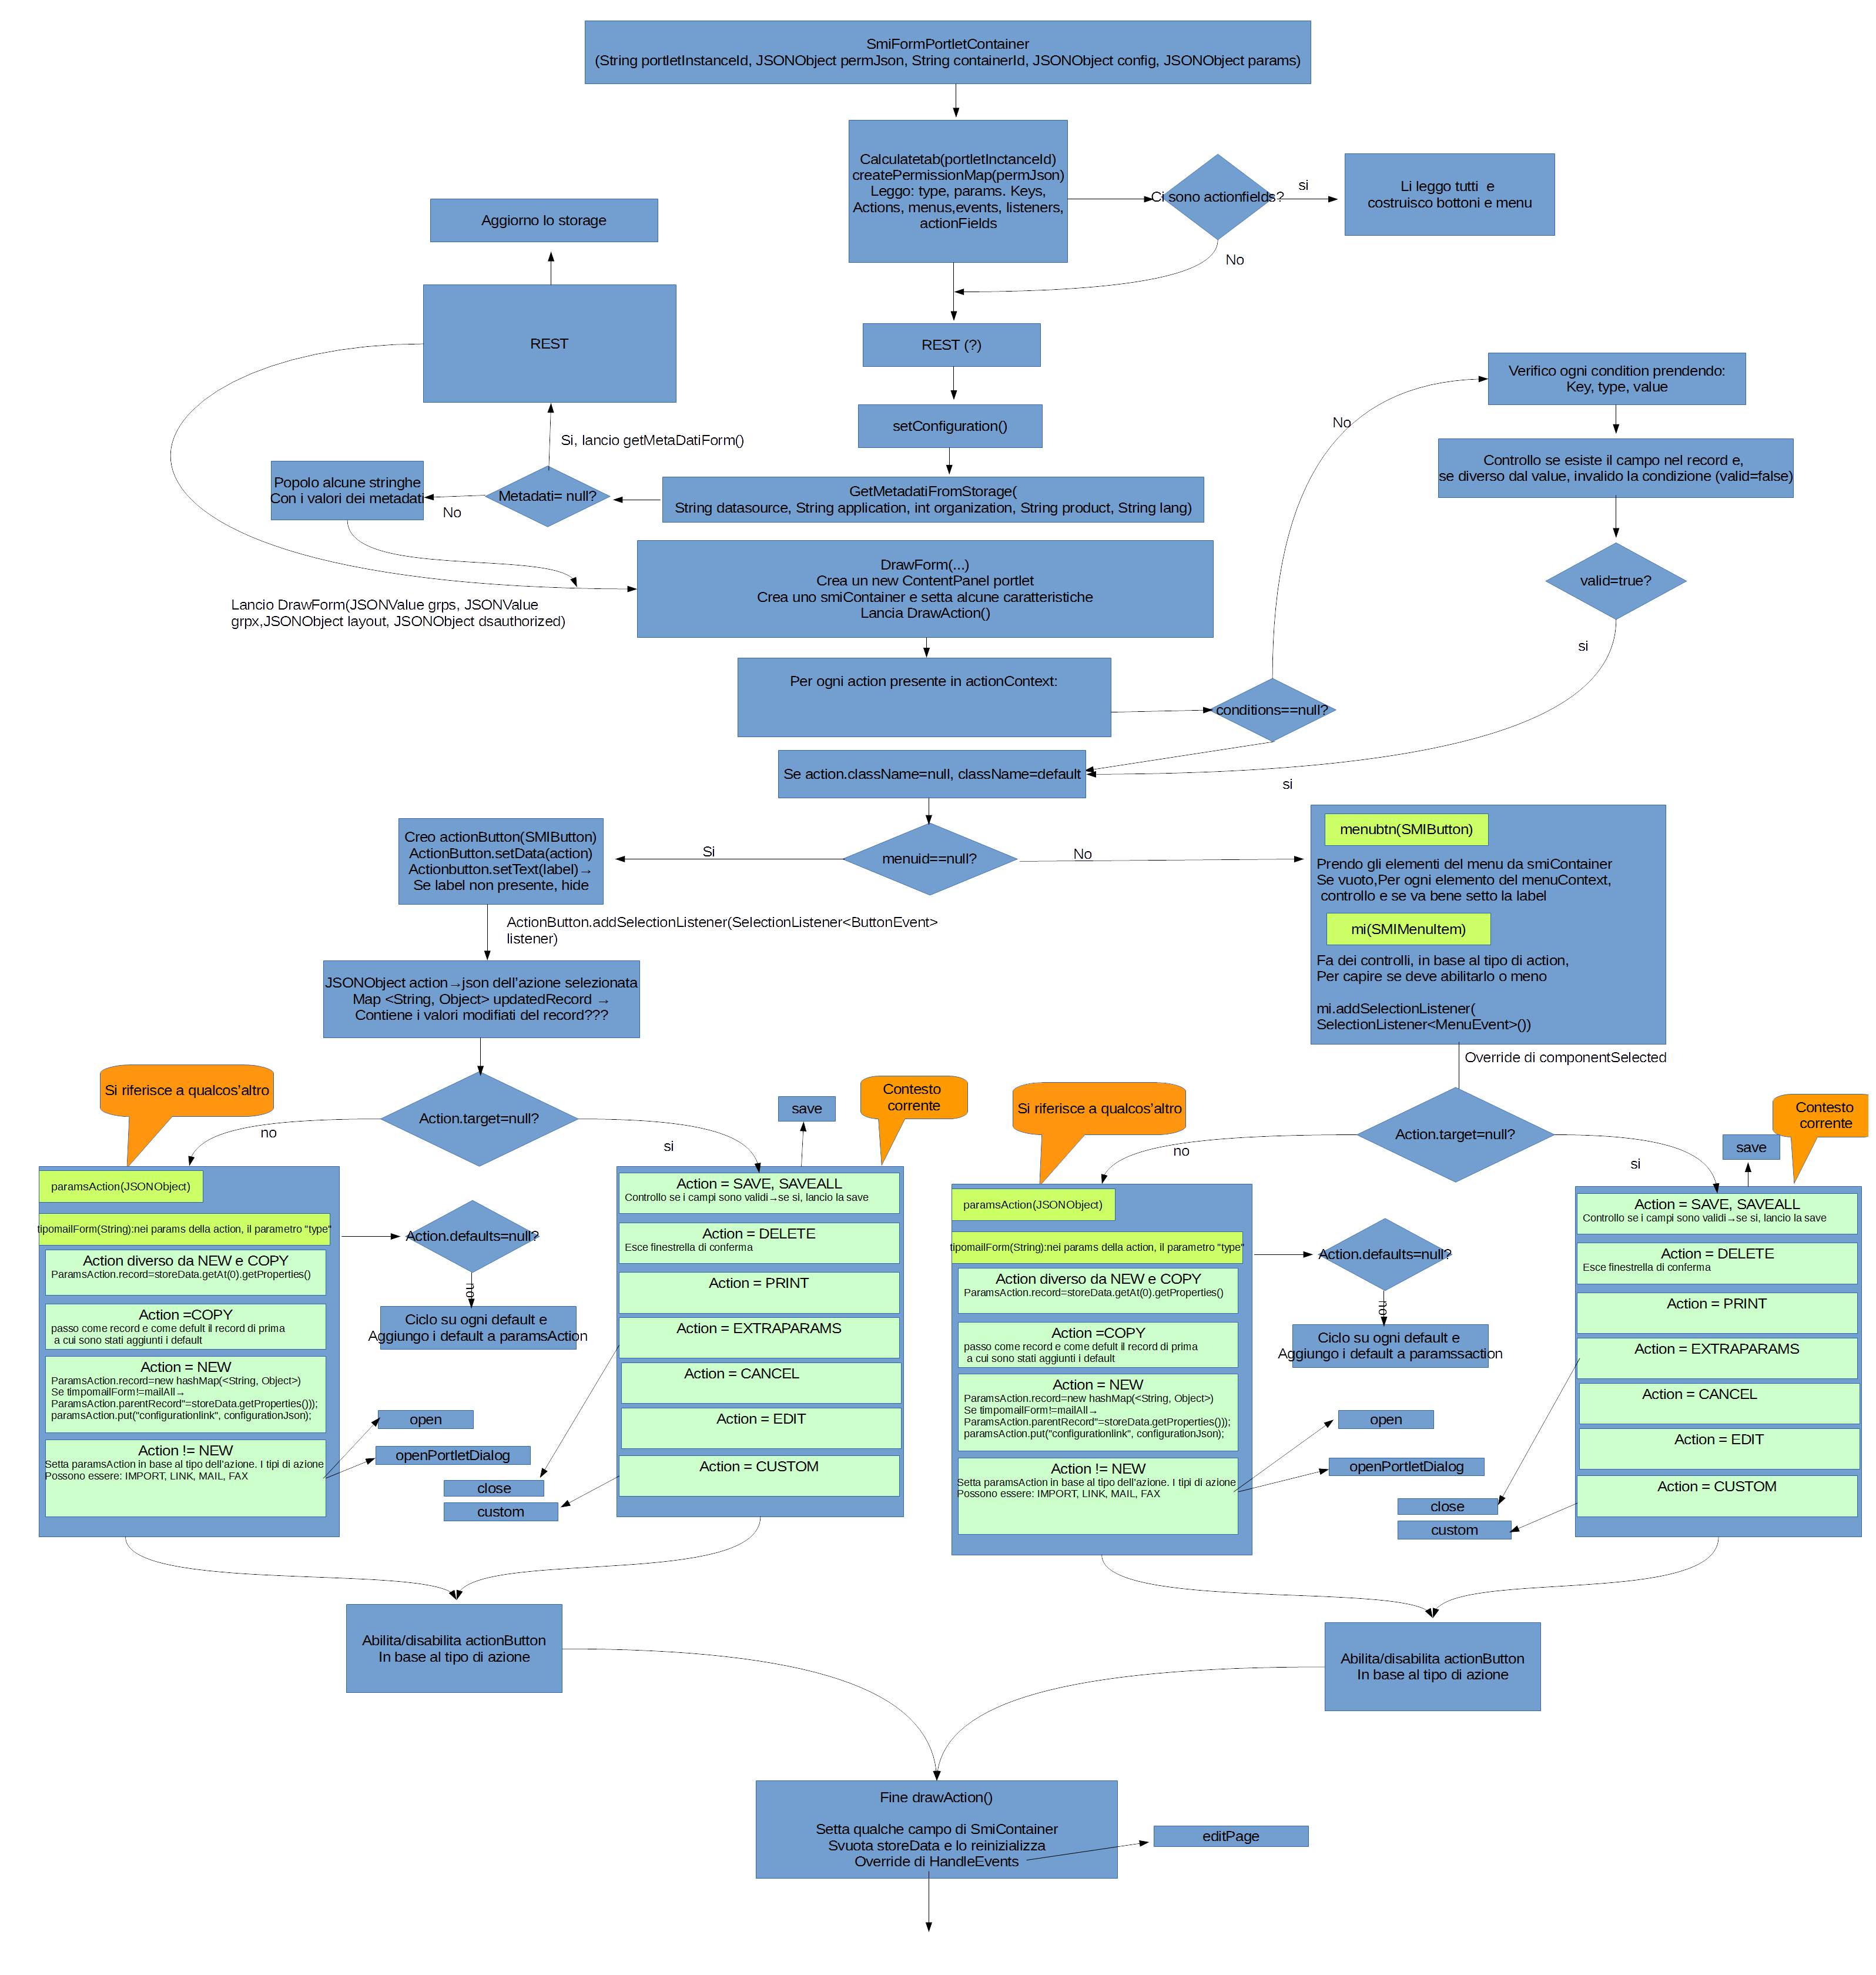
\includegraphics[width=\textwidth, height=\textheight]{diagramma-flusso}
	\caption{Diagramma di flusso della form preesistente- prima parte}
	\label{form-portlet-flow-diagram-1}
\end{figure}

\begin{figure}[p]
	\centering
	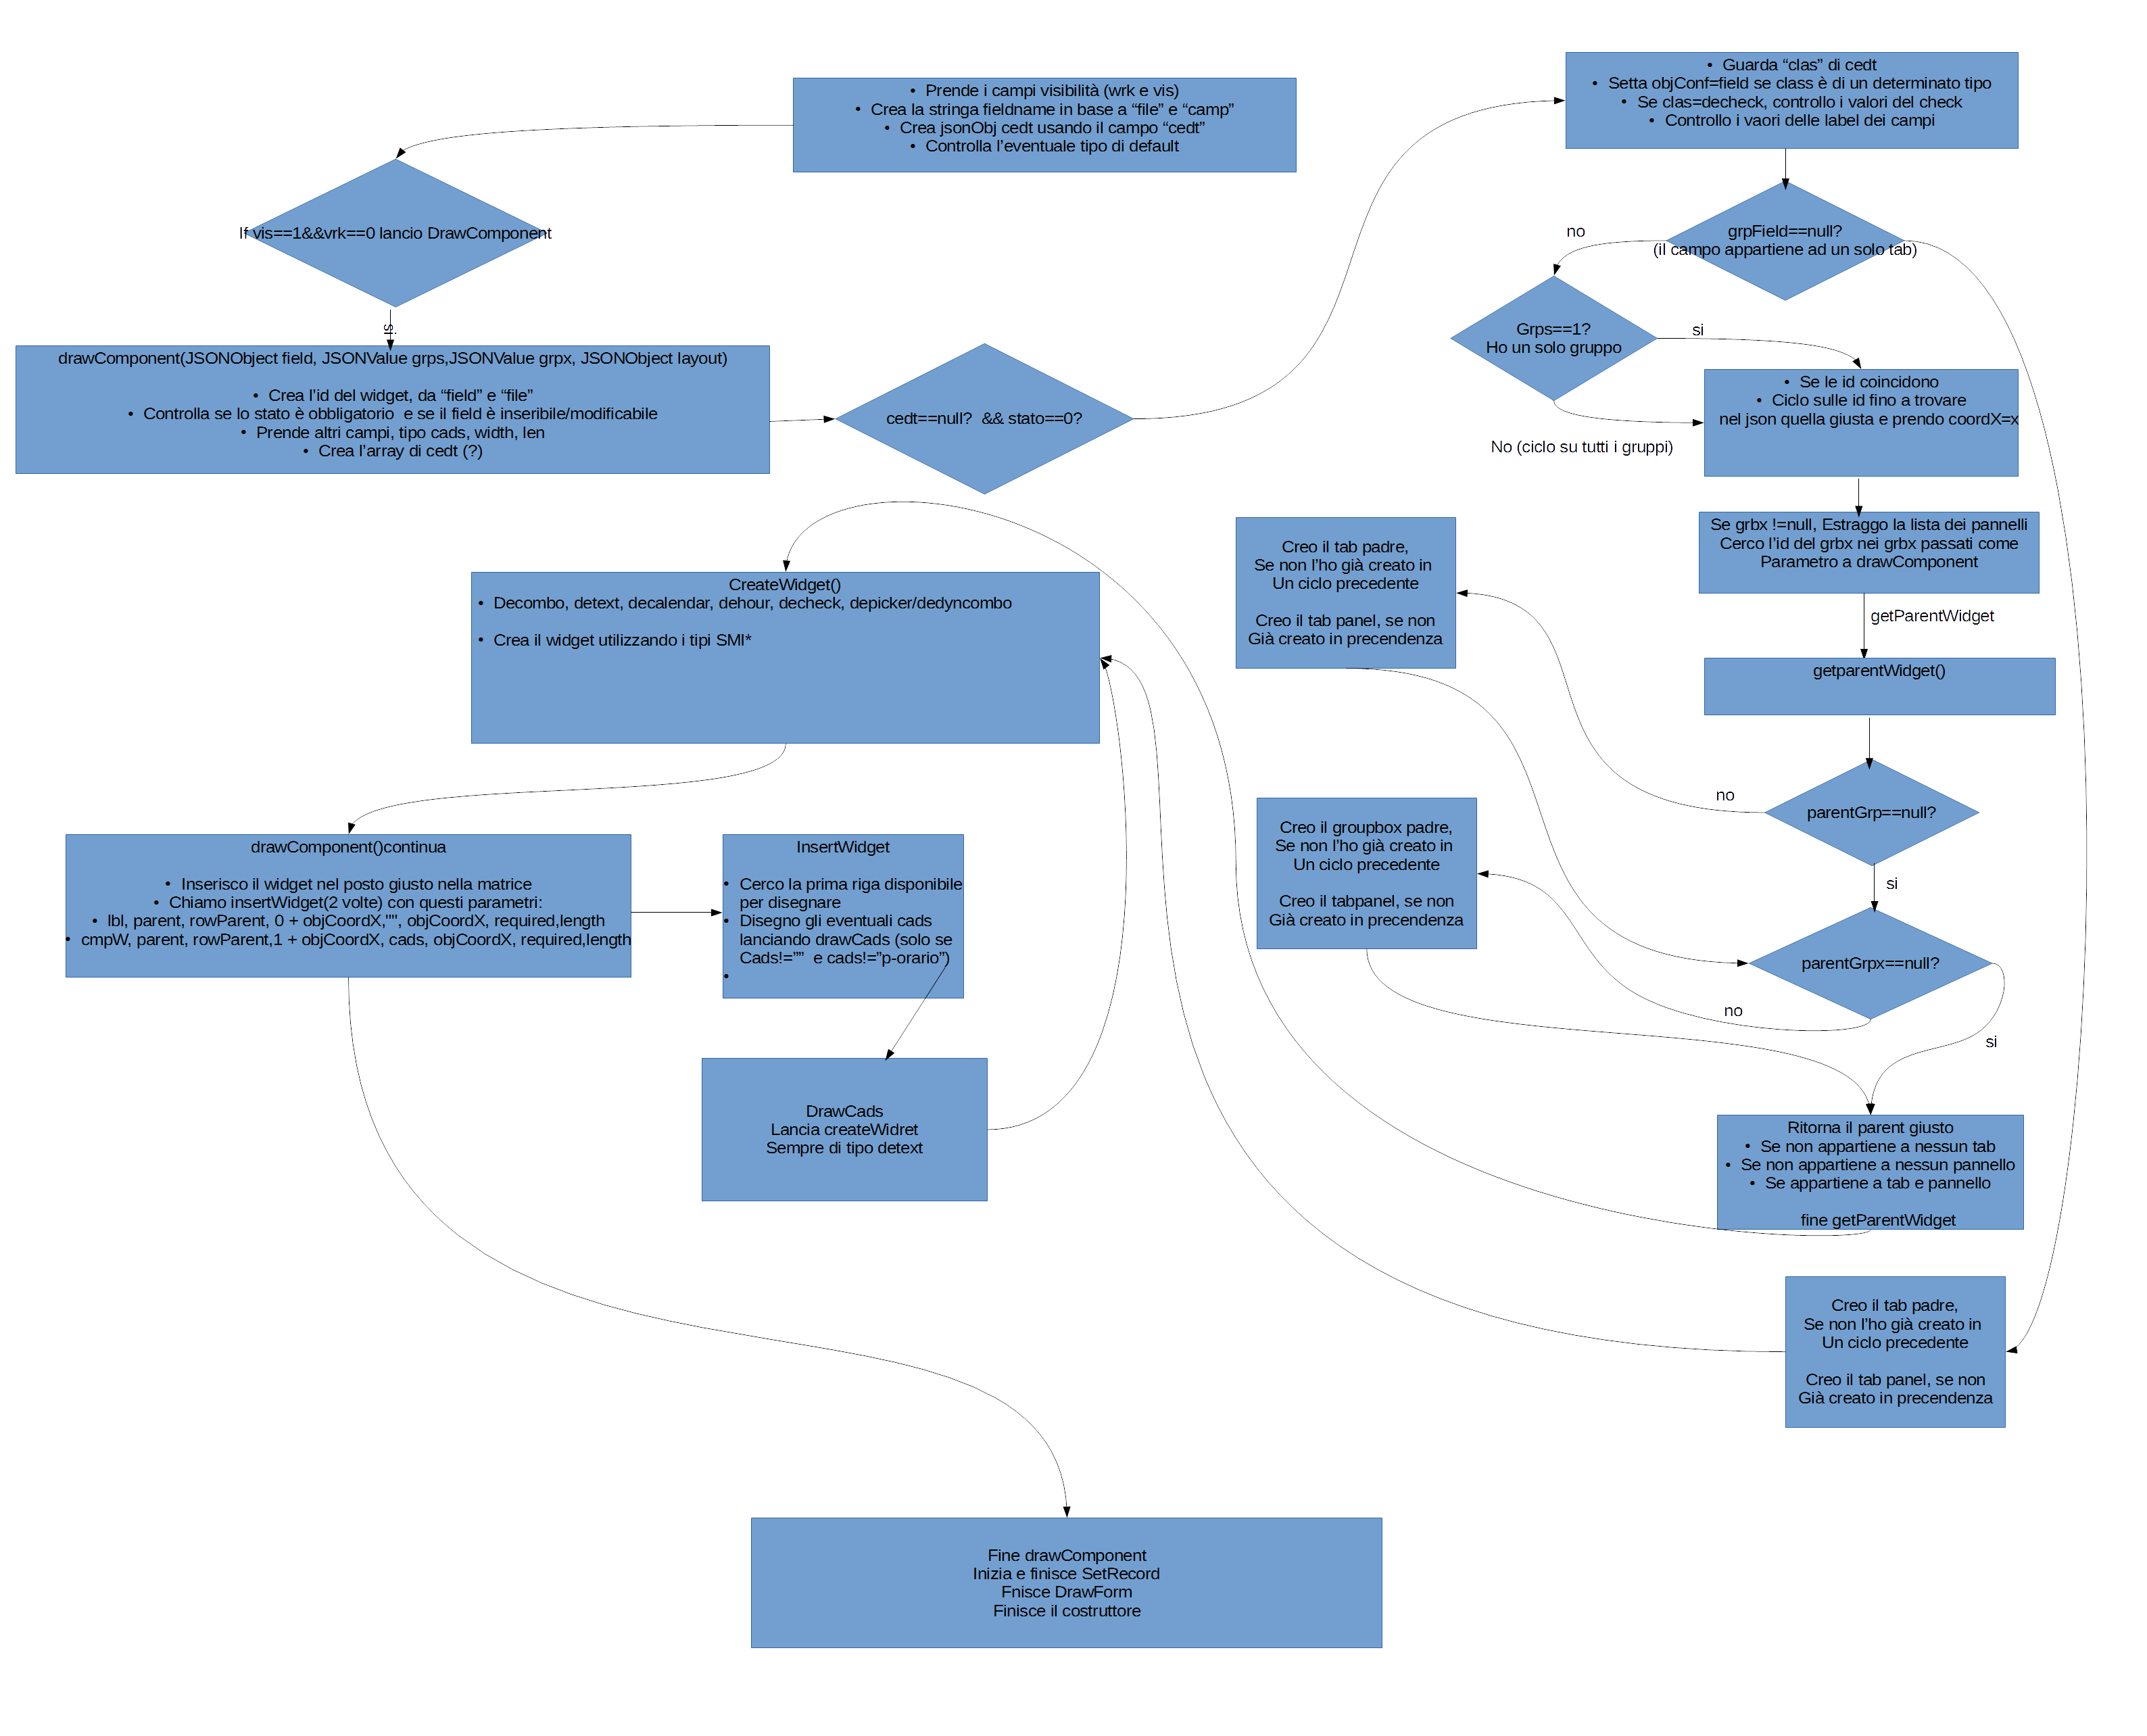
\includegraphics[width=\textwidth, height=\textheight]{diagramma-flusso-ciclo}
	\caption{Diagramma di flusso della form preesistente - seconda parte}
	\label{form-portlet-flow-diagram-2}
\end{figure}

\subsection{Descrizione del flusso}
Il flusso di esecuzione per la creazione di una form può essere essenzialmente diviso in 4 parti: 
\begin{itemize}
	\item \textbf{settaggio dei parametri e costruzione dei bottoni};
	\item \textbf{recupero del datasource};
	\item \textbf{creazione delle azioni};
	\item \textbf{creazione dei fields descritti dal datasource};
\end{itemize}
\subsubsection{Settaggio dei parametri e costruzione dei bottoni}
In questa prima parte del flusso, vengono settati alcuni parametri utili alla creazione della \gls{portlet} stessa.\\
Al costruttore della classe vengono infatti passati alcuni parametri, contenuti in oggetti di tipo String od in file JSON, contenenti informazioni quali ad esempio:
\begin{itemize}
	\item l'utente connesso con i relativi permessi;
	\item l'id della \gls{portlet};
	\item la configurazione della portlet, contenente parametri utili al recupero del datasource;
	\item il \gls{record} dei dati (vuoto nel caso di una form per l'inserimento di dati).
\end{itemize}
Dalla configurazione si prelevano poi parametri sulla presenza o meno di chiavi per il recupero di un \gls{record} in particolare, delle \gls{portlet} eventualmente in ascolto di cambiamenti e parametri che indicano la presenza di bottoni, che vengono eventualmente costruiti immediatamente.\\
\subsubsection{Recupero del datasource}
Successivamente è necessario recuperare dal server il file JSON contenente l'insieme dei campi dati da visualizzare: viene dapprima controllato se esso è già disponibile nel localStorage e, nel caso esso non fosse già stato caricato in precedenza, viene richiesto al server Tomcat.
La richiesta avviene attraverso delle chiamate \gls{restg}: %todo
\subsubsection{Creazione delle azioni}
Una volta ottenuto il datasource, è possibile passare alla costruzione delle parti che andranno ad interagire con l'utente:\\
Dapprima vengono lette dal datasource le azioni che la form può eseguire. Il flusso di esecuzione qui si dirama molto a seconda che l'azione abbia o meno una seconda \gls{portlet} target, che sia contenta o meno in un menù e comunque in base al tipo di azione che si dovrà creare.\\
I tipi di azione sono i seguenti:
\begin{itemize}
	\item \textbf{new};
	\item \textbf{copy};
	\item \textbf{import};
	\item \textbf{link};
	\item \textbf{mail};
	\item \textbf{save};
	\item \textbf{print};
	\item \textbf{delete};
	\item \textbf{custom};
\end{itemize}
I metodi invocati sono diversi per ogni azione, e si occupano della gestione della funzionalità allorché l'utente prema il relativo pulsante.
\newpage
\subsubsection{Creazione dei fields}
Infine viene eseguito un ciclo su tutti i campi dati rappresentati nel datasource. Questa è la parte più complessa del flusso in quanto ogni campo contiene avariate caratteristiche che è necessario andare a verificare per la corretta costruzione dello stesso. Esso è descritto nel datasource, con alcune variazioni (a volte piuttosto importanti) a seconda della tipologia di campo, come riportato nella figura \ref{fig:json-details}, che rappresenta i parametri relativi al campo "mail".\\  
	\begin{figure}[h]
		\centering
		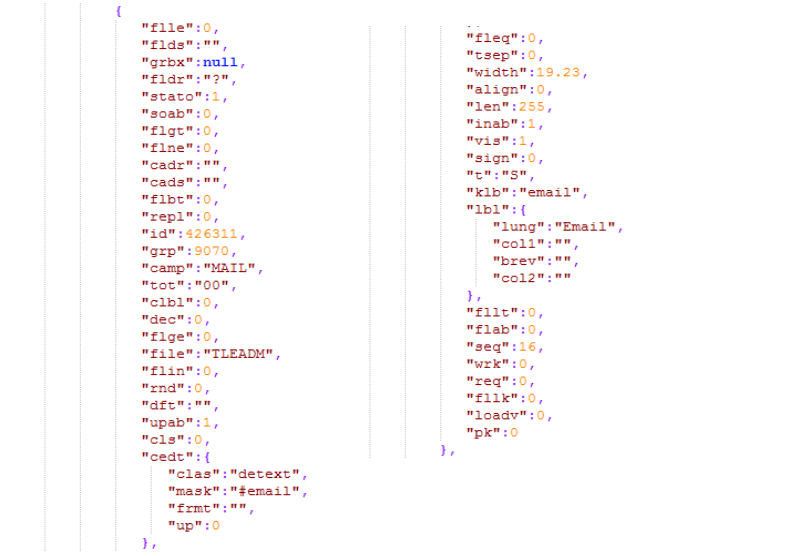
\includegraphics[height=8 cm]{json-details}
		\caption{Esempio di un campo dati come rappresentato nel datasource}
		\label{fig:json-details}
	\end{figure}
Vengono letti i campi relativi all'effettiva rappresentazione sullo schermo del campo, i premessi di scrittura, l'eventuale valore di default, che viene inserito in un particolare tipo di \gls{record} e vengono letti i valori, rappresentati in un punto differente del file, relativi al posizionamento del campo all'interno della form.\\
Vengono quindi create le tab ed i groupbox per contenere i campi.\\
Viene poi letta la tipologia di campo, che può essere
\begin{itemize}
	\item \textbf{text};
	\item \textbf{combobox};
	\item \textbf{date};
	\item \textbf{picker};
\end{itemize}
Per ognuna di queste tipologie vengono chiamati dei metodi appropriati che costruiscono il campo: il più complesso è il campo picker, che tra i suoi parametri contiene le indicazioni per il recupero dei dati che saranno poi oggetto della ricerca da parte dell'utente.\\
Infine viene effettuata un'ulteriore chiamata \gls{restg} per recuperare il record completo, tenendo anche conto dei valori di default recuperati dal ciclo appena effettuato.

\newpage